% 固定来源PDF印刷页51第15题直三棱柱及指定线段的示意重绘。
% 仅表示标号、棱与中点关系，投影比例不代表题设长度。
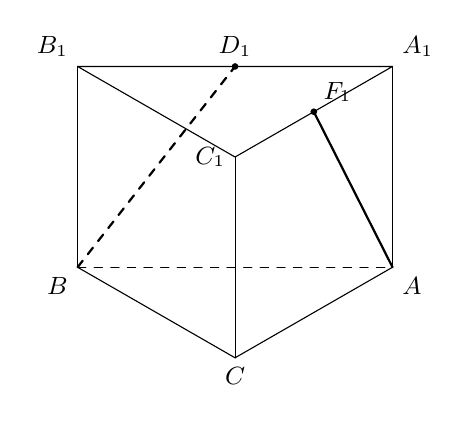
\begin{tikzpicture}[x=1cm,y=1cm,font=\small,line cap=round,line join=round]
  \coordinate (B) at (-2,0);
  \coordinate (A) at (2,0);
  \coordinate (C) at (0,-1.15);
  \coordinate (B1) at (-2,2.55);
  \coordinate (A1) at (2,2.55);
  \coordinate (C1) at (0,1.4);
  \coordinate (D1) at (0,2.55);
  \coordinate (F1) at (1,1.975);

  % Bottom triangle: the rear edge is hidden in the source projection.
  \draw[dashed] (B)--(A);
  \draw (B)--(C)--(A);
  % Top triangle and lateral edges of the right prism.
  \draw (B1)--(A1)--(C1)--cycle;
  \draw (B)--(B1) (A)--(A1) (C)--(C1);
  % The requested segments BD_1 and AF_1.
  \draw[dashed,thick] (B)--(D1);
  \draw[thick] (A)--(F1);

  \fill (D1) circle (1.2pt) (F1) circle (1.2pt);
  \node[above left] at (B1) {$B_1$};
  \node[above right] at (A1) {$A_1$};
  \node[left] at (C1) {$C_1$};
  \node[above] at (D1) {$D_1$};
  \node[above right] at (F1) {$F_1$};
  \node[below left] at (B) {$B$};
  \node[below right] at (A) {$A$};
  \node[below] at (C) {$C$};
\end{tikzpicture}
